\subsection{Matlab Code}

\usemintedstyle{tango}

\inputminted[breaklines]{Matlab}{./Code/AmplitudeModulator.m}

\subsection{Schematic: Power Supply}
\begin{figure}[H]
    \centering
    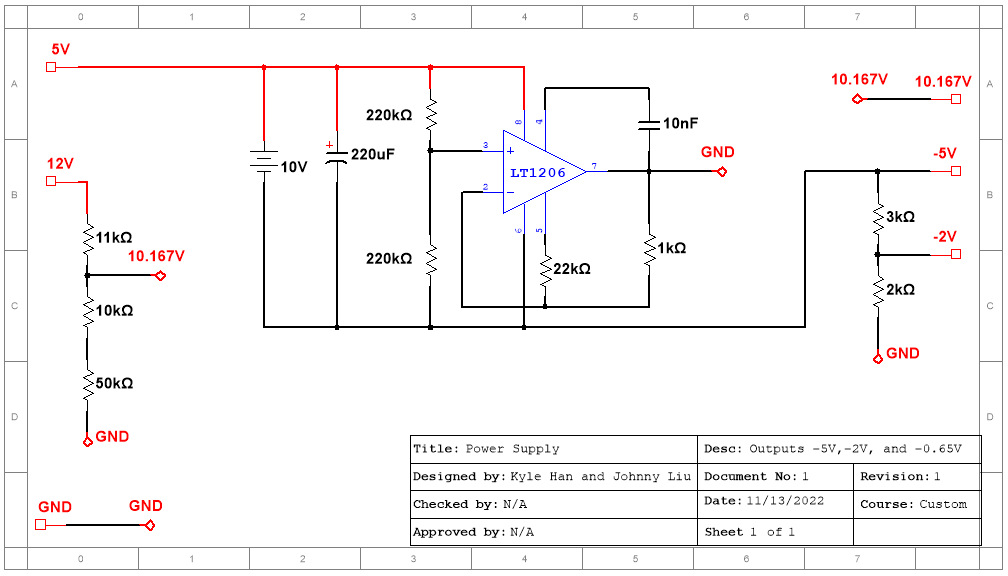
\includegraphics[width = 1\textwidth]{Appendices/ESE342_Design1_Power_Supply.png}
    \caption{Power Supply Circuit to obtain 10.167V, -2V, and -5V}
    \label{fig:PowerSupply}
\end{figure}

\subsection{Schematic: Amplitude Modulator}
\begin{figure}[H]
    \centering
    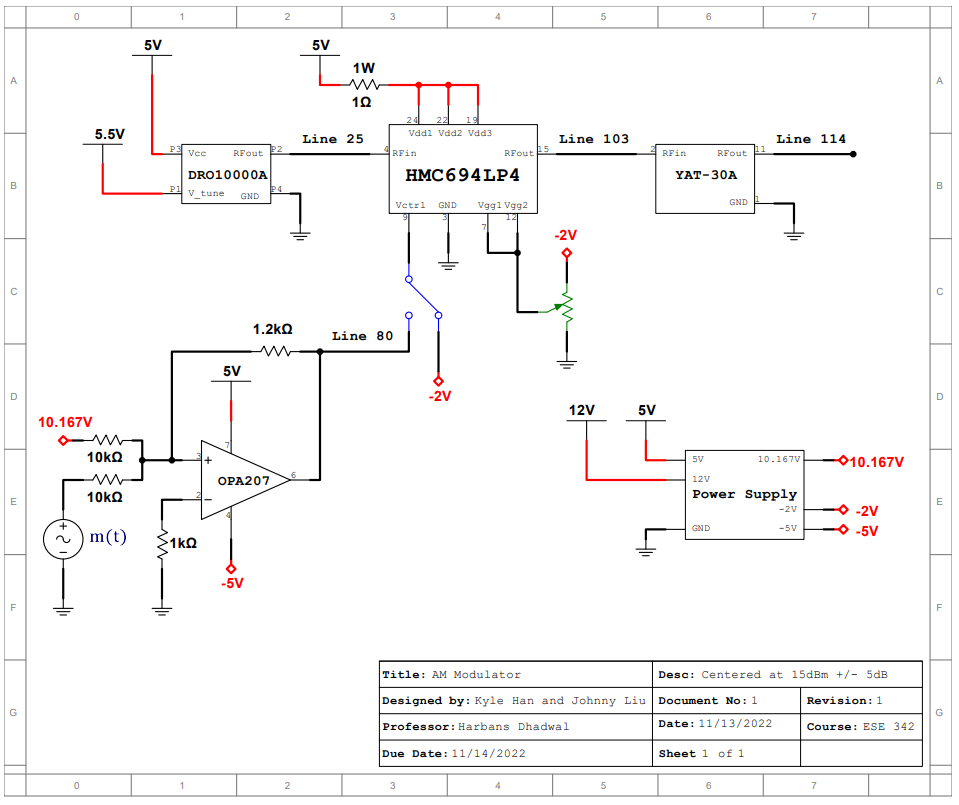
\includegraphics[width = 1\textwidth]{ESE342_Design1.png}
    \caption{Amplitude Modulator Circuit for 15dBm $\pm$5dB swing. Labelled wires for inputs and outputs for }
    \label{fig:AMCircuit}
\end{figure}https://www.overleaf.com/project/636a79a82392e04240efe040

\subsection{Datasheets}
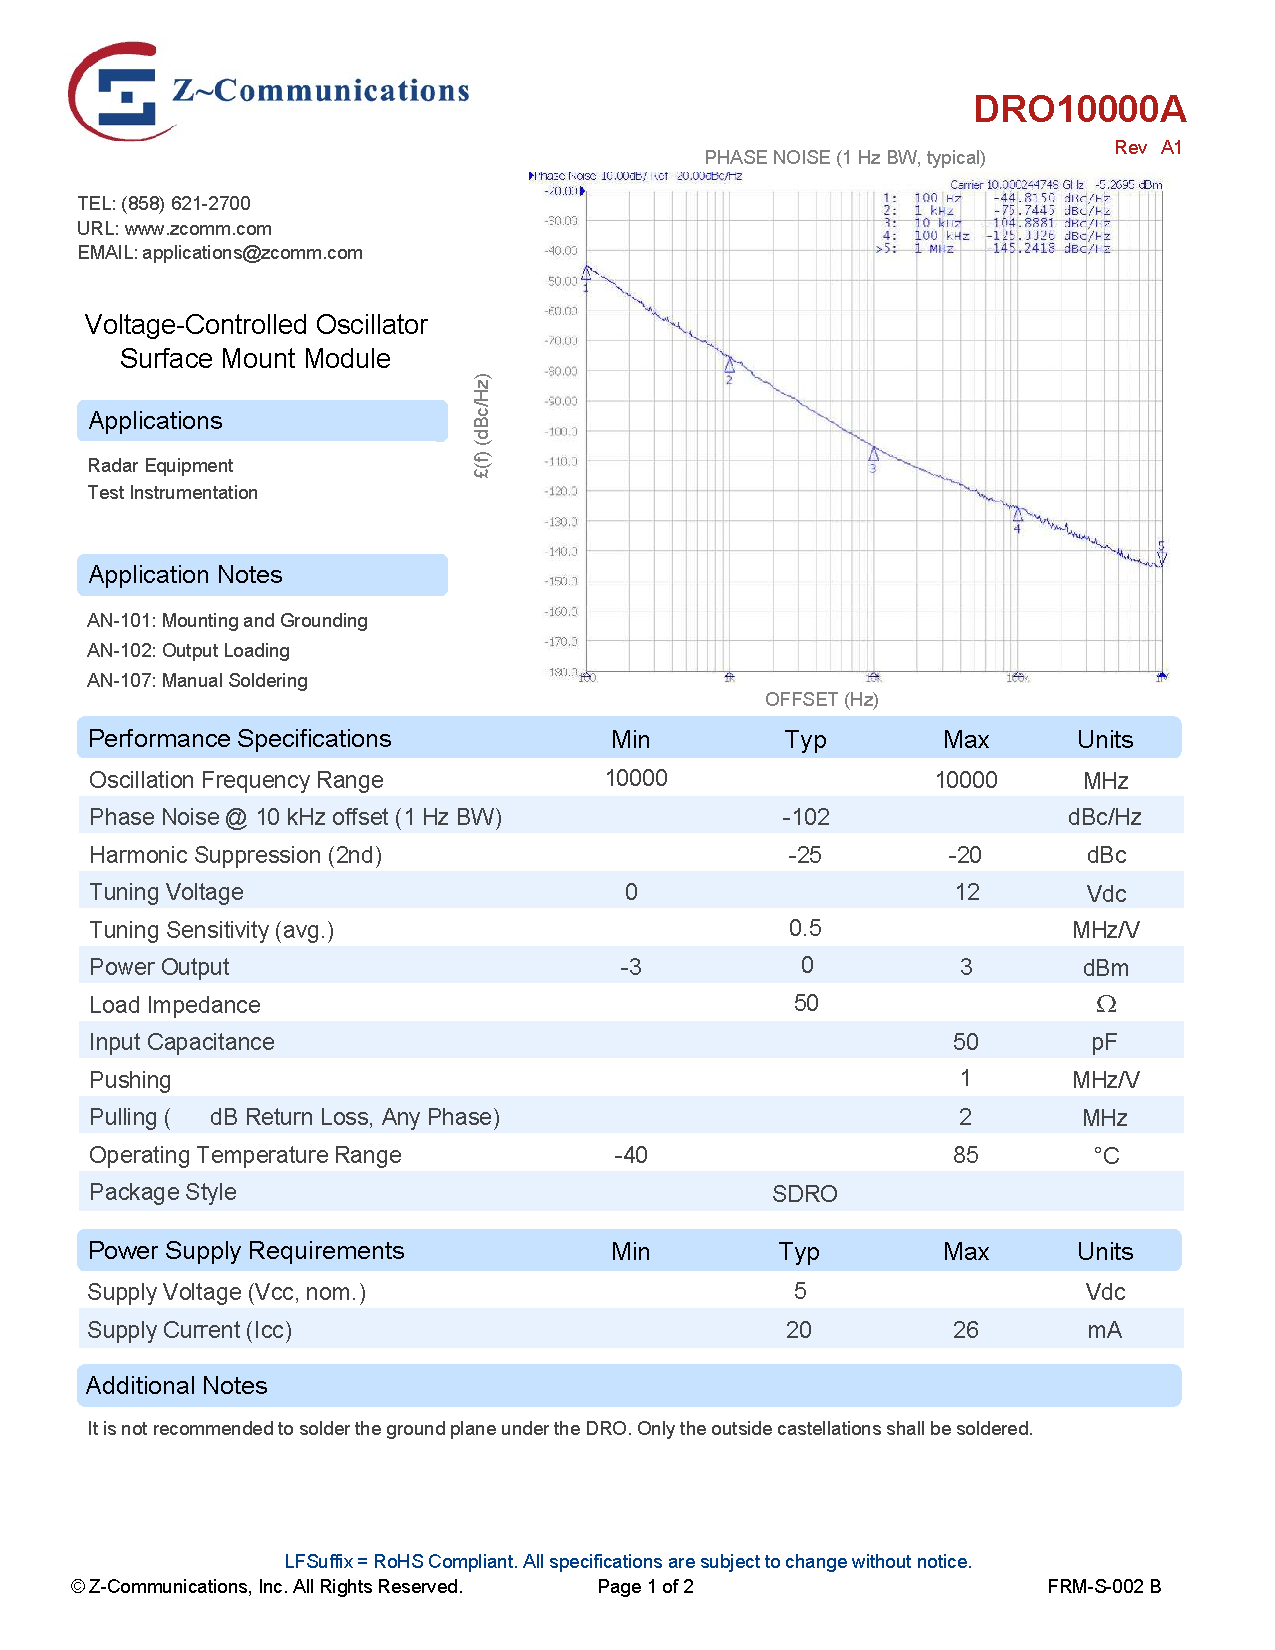
\includepdf[pages=-,pagecommand={},width=\textwidth]{DRO10000A.pdf}
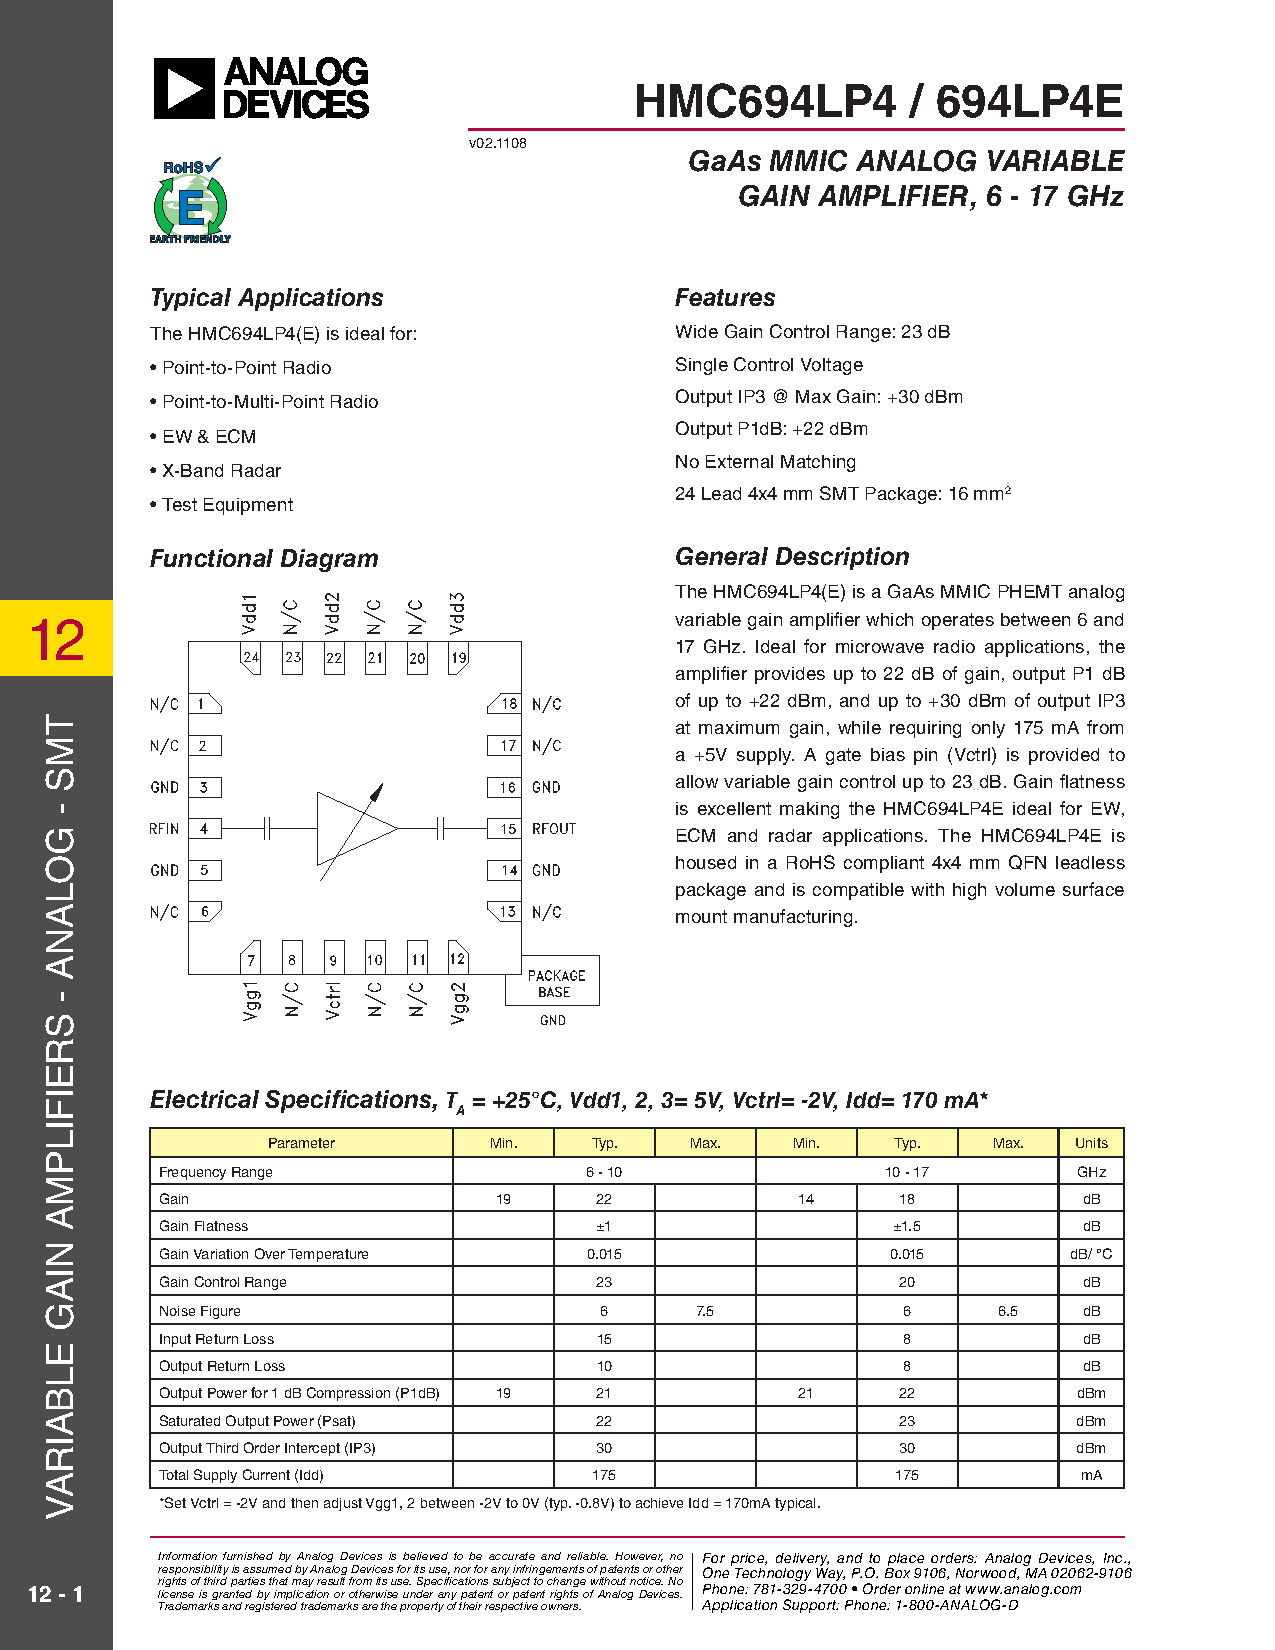
\includepdf[pages=-,pagecommand={},width=\textwidth]{hmc694.pdf}
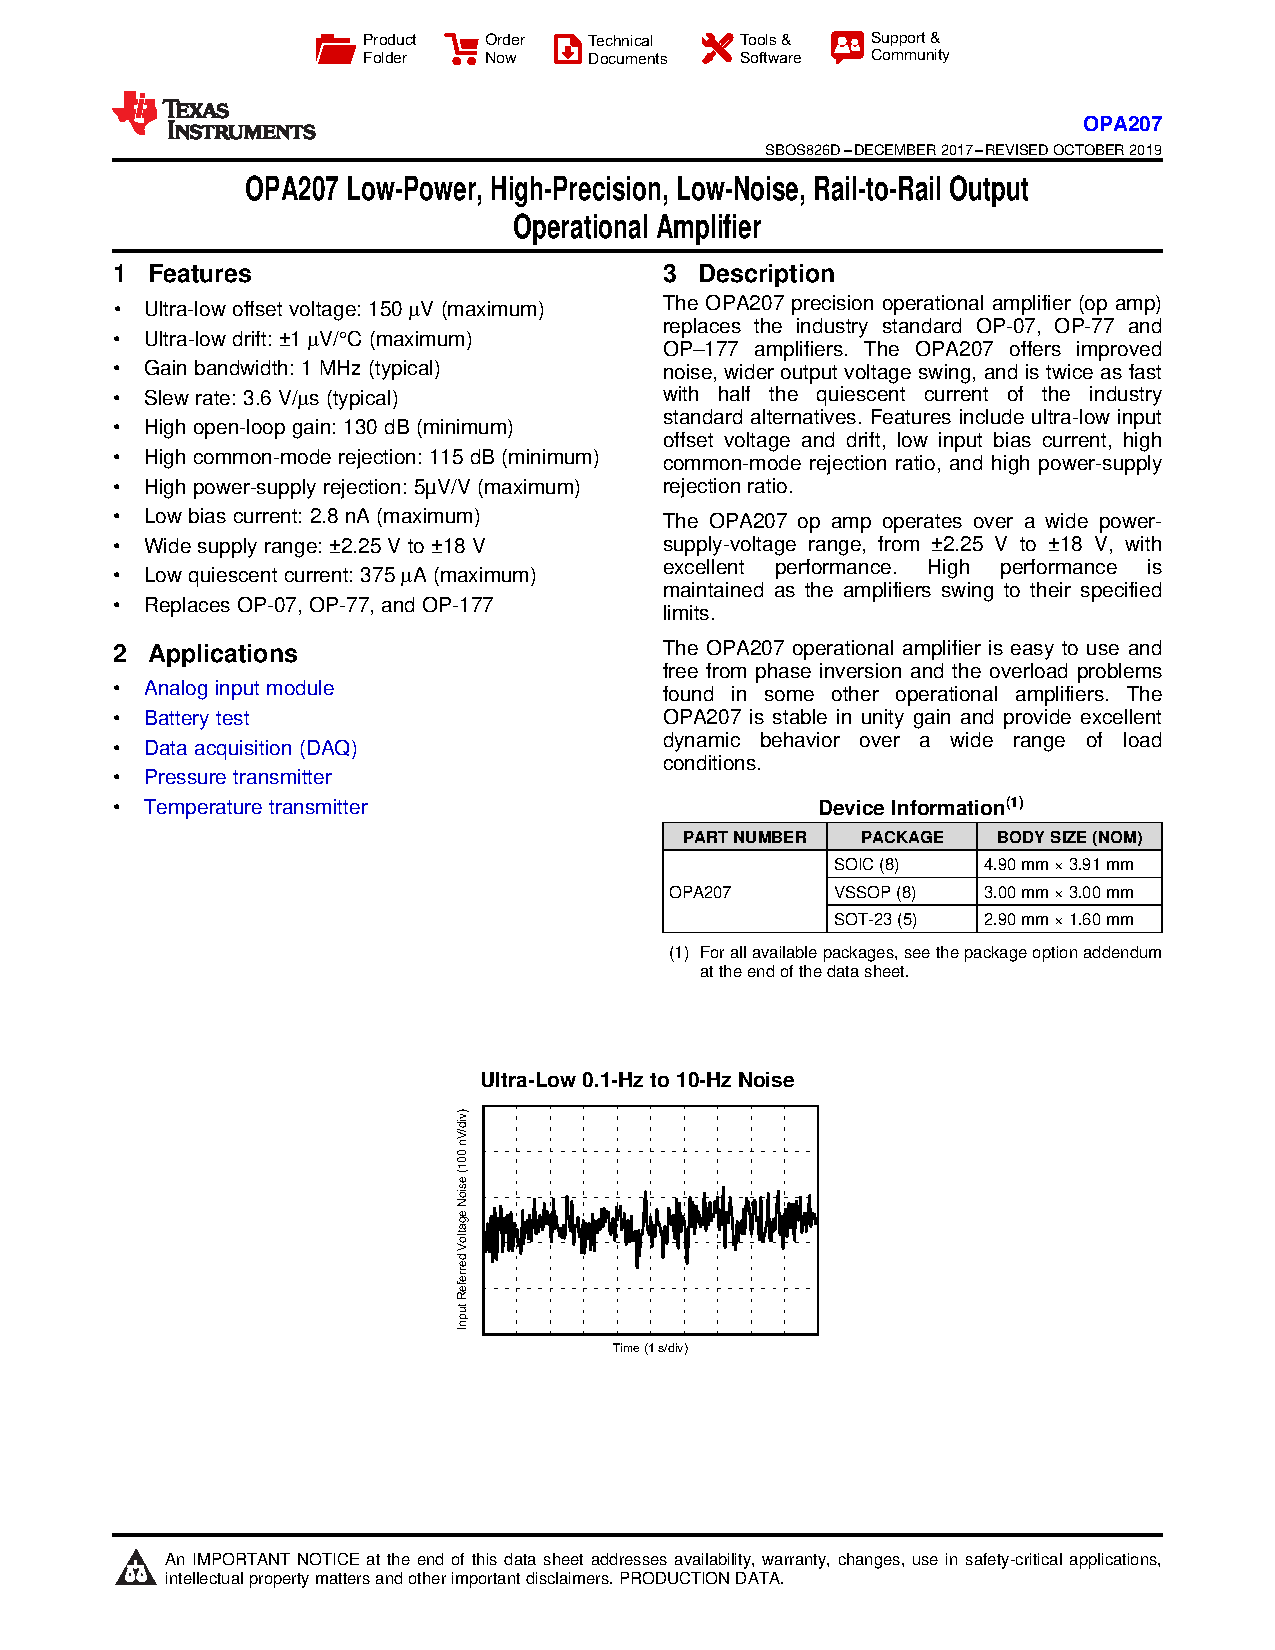
\includepdf[pages=-,pagecommand={},width=\textwidth]{opa207.pdf}
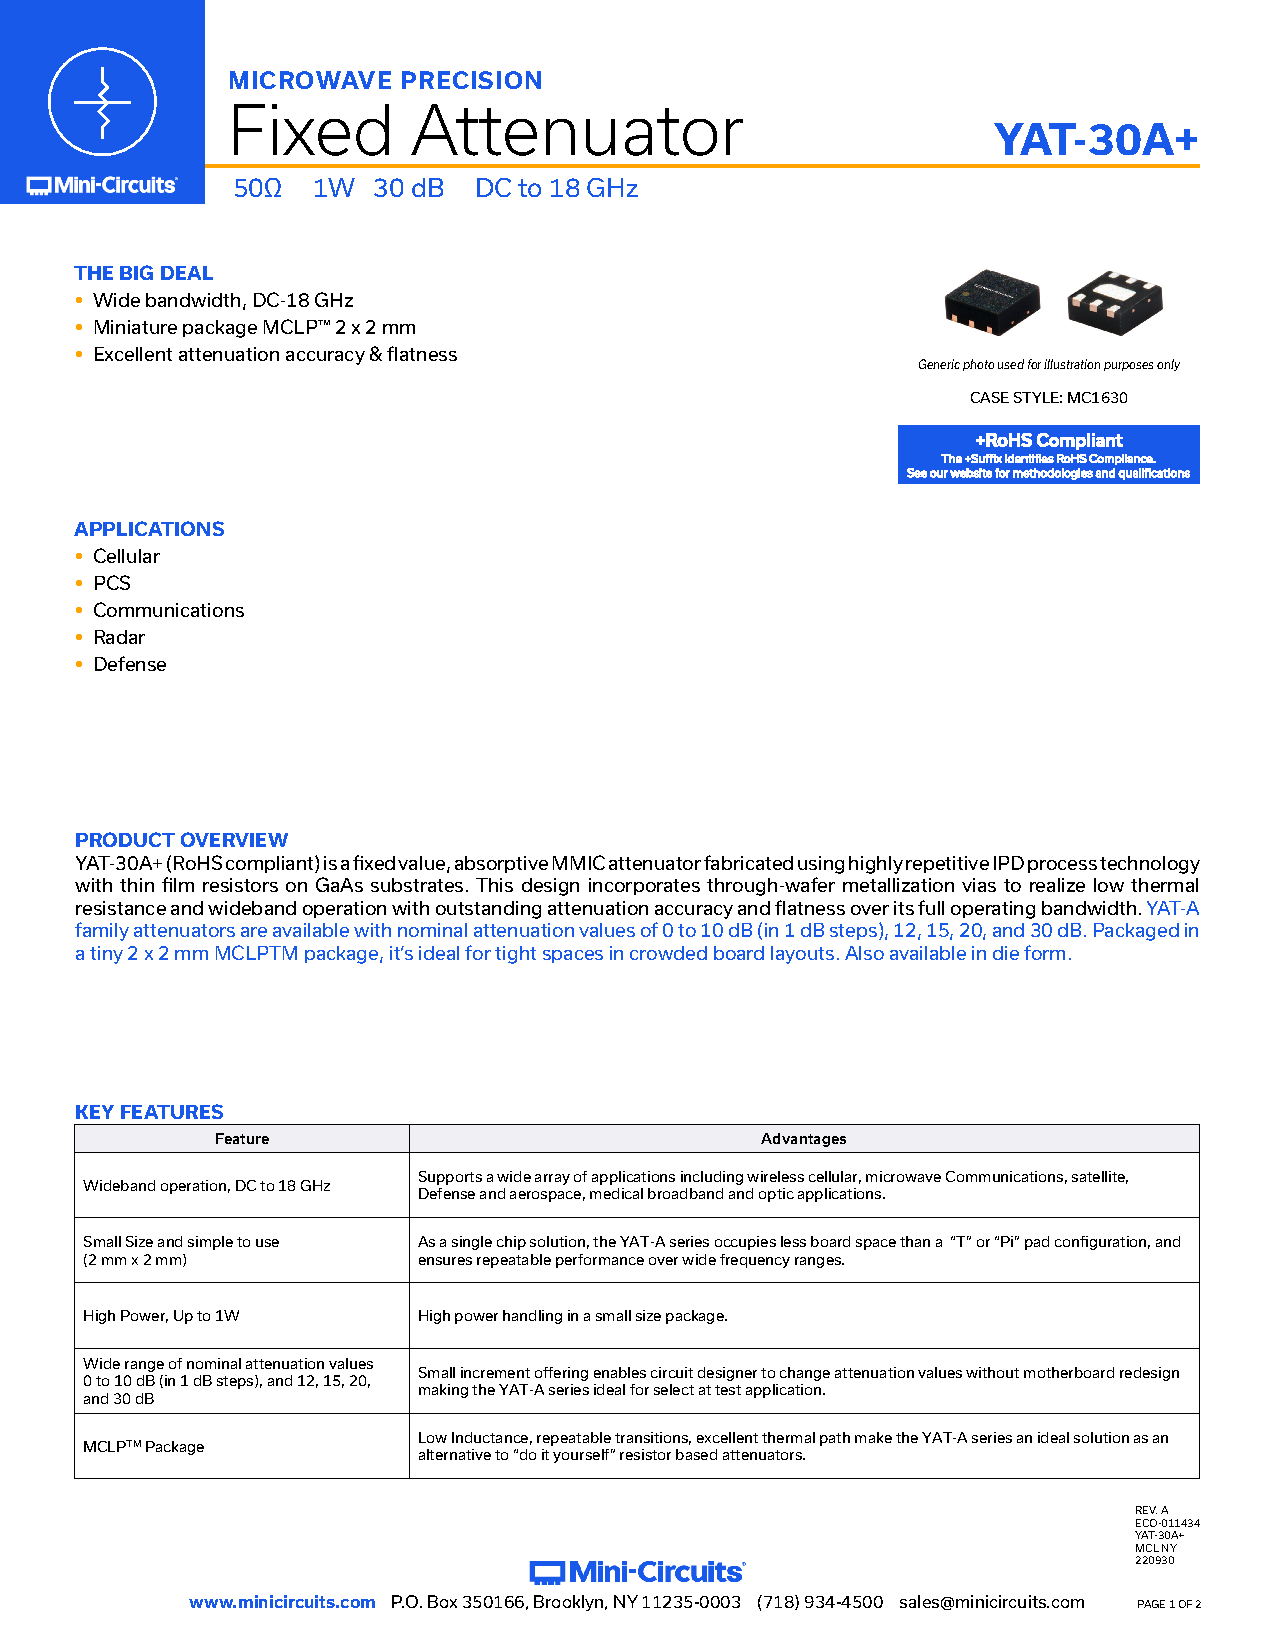
\includepdf[pages=-,pagecommand={},width=\textwidth]{YAT-30A+.pdf}